Avendo stabilito i principi del cloud computing e le ragioni della scelta di AWS, questo capitolo si addentra negli aspetti pratici dell'implementazione di un'infrastruttura sicura e scalabile su AWS per una startup fintech. Verranno presentati esempi concreti di configurazioni e utilizzi dei servizi AWS, focalizzandosi sulle best practice di sicurezza applicabili in un contesto con risorse limitate ma requisiti elevati, tipico di una startup nel settore finanziario.

\section{Configurazione Attuale dell'Ambiente AWS}
\label{sec:aws_infrastruttura_attuale}

L'infrastruttura cloud della startup è stata realizzata utilizzando i servizi di Amazon Web Services (AWS), con le operazioni principali concentrate nella regione geografica \texttt{eu-south-1} (Milano). L'account AWS utilizzato ha ID \texttt{478291635847} ed è configurato con una separazione degli ambienti: uno dedicato allo sviluppo, chiamato \texttt{Finanz-Dev}, e uno per l'applicazione in uso dagli utenti finali, chiamato \texttt{Finanz-Prod}. Questa divisione è una buona pratica per testare nuove funzionalità senza impattare il servizio principale.

Il cuore dell'infrastruttura applicativa è \textbf{AWS Elastic Beanstalk}. Si tratta di un servizio AWS che semplifica il processo di rilascio e gestione delle applicazioni, in questo caso denominate "Finanz". L'ambiente di sviluppo utilizza la configurazione \texttt{finanz-dev-v2} mentre quello di produzione opera su \texttt{finanz-prod-v1.3}. Elastic Beanstalk si occupa di creare e configurare automaticamente le risorse necessarie, come le macchine virtuali \textbf{Amazon EC2} (principalmente di tipo \texttt{t3a.small} per l'ambiente di sviluppo e \texttt{t3a.medium} per la produzione, adatte per carichi di lavoro di piccole e medie dimensioni con un buon rapporto prezzo-prestazioni). L'ambiente di sviluppo gestisce tipicamente 1-2 istanze, mentre quello di produzione ne mantiene attive 3-5 durante i picchi di utilizzo. Inoltre, automatizza il bilanciamento del carico (distribuzione del traffico tra più macchine per evitare sovraccarichi) e l'auto-scaling (aumento o diminuzione automatica delle macchine virtuali in base al traffico). Per l'ambiente di produzione, un \textbf{Application Load Balancer (ALB)} denominato \texttt{finanz-prod-alb-1284567}, un tipo specifico di bilanciatore di carico, distribuisce le richieste degli utenti alle istanze EC2, aumentando così la disponibilità (il servizio rimane accessibile anche se una macchina ha problemi) e la resilienza (capacità di recupero da guasti).

Per la gestione dei dati, Finanz utilizza \textbf{Amazon RDS for PostgreSQL}. RDS (Relational Database Service) è un servizio che semplifica la configurazione e la manutenzione di database relazionali nel cloud. Sono state create due istanze database separate: una per lo sviluppo (\texttt{finanz-dev-db.cluster-cx4s7k9m2qla.eu-south-1.rds.amazonaws.com} di tipo \texttt{db.t4g.micro}, più piccola ed economica) e una per la produzione (\texttt{finanz-prod-db.cluster-cx4s7k9m2qlb.eu-south-1.rds.amazonaws.com} di tipo \texttt{db.t4g.small}). Durante la fase di sviluppo ho constatato che l'istanza di sviluppo gestisce circa 50-100 connessioni simultanee con un database di ~2GB, mentre quella di produzione arriva a gestire fino a 500 connessioni con un database di ~15GB. L'istanza di produzione è configurata in modalità \textbf{Multi-AZ} (Multi-Availability Zone): ciò significa che una copia del database viene mantenuta sincronizzata in una diversa zona di disponibilità (un data center fisicamente separato all'interno della stessa regione AWS). Questa configurazione garantisce che il database rimanga operativo anche in caso di problemi in una singola zona di disponibilità. Entrambe le istanze RDS sono protette da crittografia, che rende i dati illeggibili senza la chiave corretta; queste chiavi sono gestite dal servizio \textbf{AWS KMS (Key Management Service)} con la chiave specifica \texttt{arn:aws:kms:eu-south-1:478291635847:key/12345678-1234-1234-1234-123456789012}.

La rete virtuale privata della startup è definita tramite \textbf{Amazon VPC (Virtual Private Cloud)}, chiamato "Finanz-vpc" con CIDR block \texttt{10.0.0.0/16}. Un VPC permette di creare una sezione isolata della cloud AWS dove lanciare le proprie risorse. All'interno di questo VPC, lo spazio di indirizzi IP è diviso in \textbf{subnet} (sottoreti). Alcune subnet sono configurate come pubbliche (subnet \texttt{10.0.1.0/24} e \texttt{10.0.2.0/24}, accessibili da Internet) e altre come private (subnet \texttt{10.0.10.0/24}, \texttt{10.0.11.0/24} e \texttt{10.0.12.0/24}, isolate da Internet, per una maggiore sicurezza delle risorse applicative). Queste subnet sono distribuite su diverse \textbf{Availability Zones} (\texttt{eu-south-1a}, \texttt{eu-south-1b}, \texttt{eu-south-1c}), che sono data center fisicamente distinti all'interno della regione di Milano, per migliorare la resilienza dell'intera infrastruttura. La connettività verso Internet è fornita da un \textbf{Internet Gateway} con ID \texttt{igw-0a1b2c3d4e5f67890}. Inoltre, è presente un \textbf{VPC Endpoint per S3} con ID \texttt{vpce-1a2b3c4d5e6f7g8h9}: si tratta di un meccanismo che permette alle risorse all'interno del VPC (come le istanze EC2) di comunicare con il servizio di storage S3 utilizzando la rete privata di AWS, senza passare per l'Internet pubblico, migliorando sicurezza e prestazioni.

\textbf{Amazon S3 (Simple Storage Service)} è un servizio di storage versatile, utilizzato da Finanz per diversi scopi:
\begin{itemize}
    \item Archiviazione dei file di log (registri delle attività) generati dalle applicazioni Elastic Beanstalk e dalle istanze EC2 nel bucket \texttt{finanz-logs-478291635847}.
    \item Salvataggio degli "artefatti", ovvero i file compilati e pronti per il rilascio, prodotti da \textbf{AWS CodePipeline} nel bucket \texttt{finanz-artifacts-eu-south-1}. Quest'ultimo è un servizio che automatizza le fasi di build, test e rilascio del software (un processo noto come CI/CD - Continuous Integration/Continuous Deployment).
    \item Hosting di file statici (immagini, video, file CSS, JavaScript) per le applicazioni web "Finanz" nel bucket \texttt{finanz-static-assets}, rendendoli accessibili agli utenti via web attraverso CloudFront distribution \texttt{E1A2B3C4D5E6F7}.
\end{itemize}
Per proteggere gli artefatti archiviati in S3, viene richiesta la crittografia lato server (i dati vengono crittografati da AWS prima di essere salvati) utilizzando chiavi gestite da KMS, e si impone l'uso di connessioni sicure HTTPS tramite una bucket policy che nega esplicitamente le richieste HTTP non sicure.

Per automatizzare il rilascio del software, Finanz utilizza \textbf{AWS CodePipeline} insieme ad \textbf{AWS CodeBuild} (un servizio che compila il codice sorgente ed esegue test). Queste pipeline si integrano con Elastic Beanstalk per aggiornare le applicazioni in modo controllato. Le notifiche importanti relative agli ambienti Elastic Beanstalk (ad esempio, problemi di deployment o aggiornamenti di stato) vengono inviate tramite \textbf{AWS SNS (Simple Notification Service)}, un servizio di messaggistica e notifica.

Infine, la gestione degli utenti e dei loro permessi di accesso alle risorse AWS è organizzata in modo strutturato. \textbf{AWS Organizations} permette di gestire più account AWS sotto un'unica organizzazione; in questo caso, l'account analizzato è quello principale (management account). Per l'accesso degli utenti, viene utilizzato \textbf{AWS IAM Identity Center (precedentemente noto come AWS SSO)}, che consente di gestire centralmente gli accessi e di utilizzare, ad esempio, le stesse credenziali aziendali per accedere ad AWS. I permessi specifici vengono concessi ai servizi AWS tramite \textbf{Ruoli IAM} (Identity and Access Management), come ad esempio il ruolo \texttt{aws-elasticbeanstalk-ec2-role} usato dalle istanze EC2. Questo approccio segue il principio del "minimo privilegio", ovvero concedere solo i permessi strettamente necessari per svolgere una determinata funzione, riducendo i rischi in caso di problemi di sicurezza.

\begin{figure}[h] % opzioni di posizionamento comuni: h=here, t=top, b=bottom, p=page of floats
  \centering
  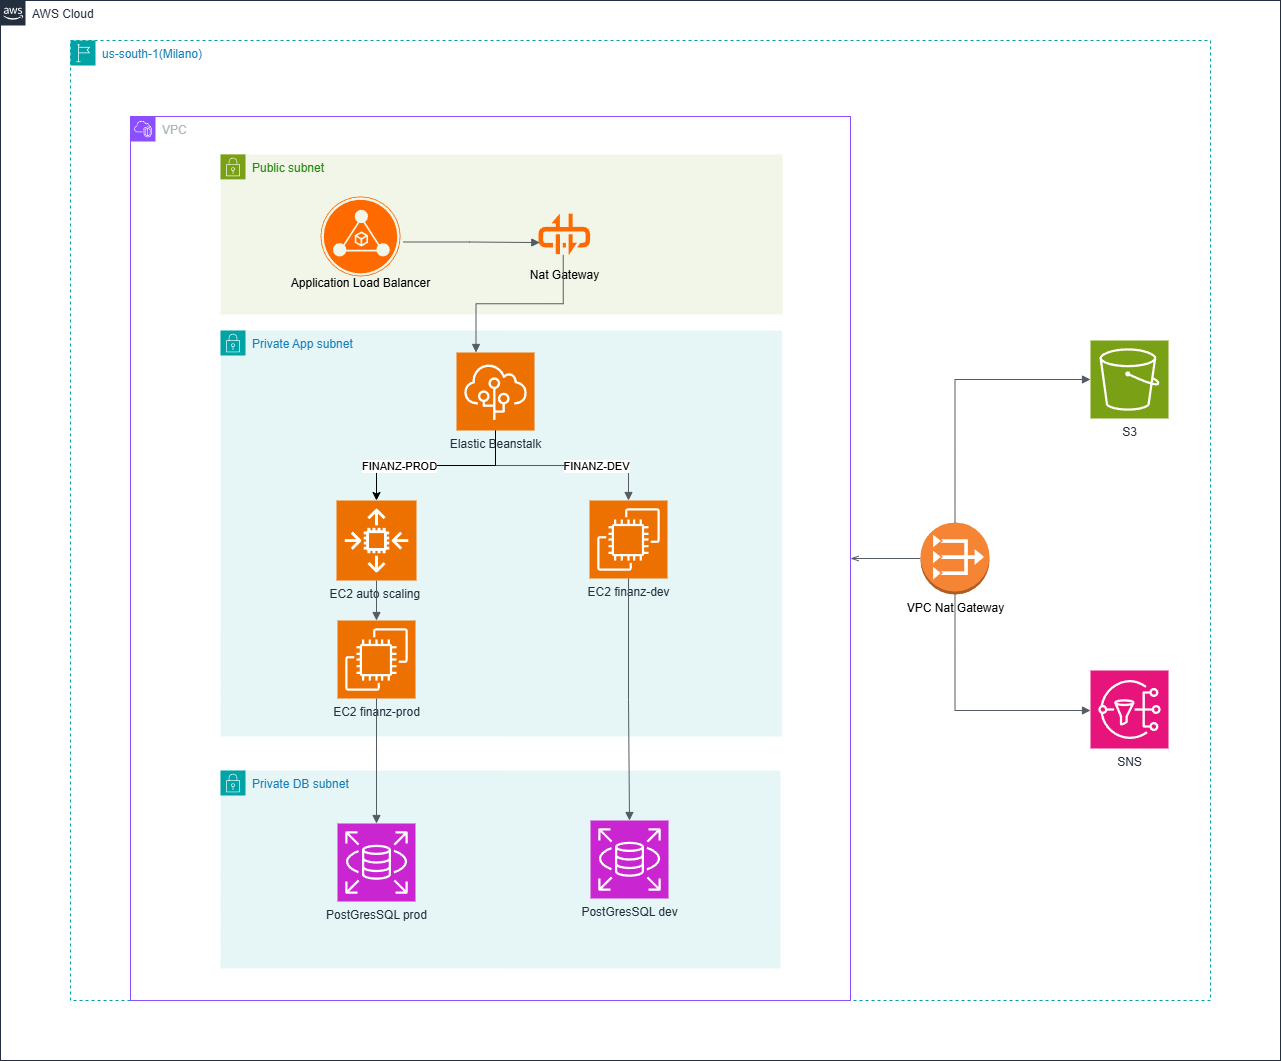
\includegraphics[width=0.8\textwidth]{aws_struttura} % Aggiunto [width=...] come esempio per scalare l'immagine
  \caption{Descrizione della struttura attuale in AWS.} % Aggiungi una didascalia significativa
  \label{fig:aws_struttura_attuale} % Label DOPO \caption, con un prefisso come 'fig:'
\end{figure}

\section{Principi di Sicurezza per la Gestione delle Identità e degli Accessi e Analisi del Contesto Attuale}
\label{sec:principi-identita-accessi}
\subsection{Implementazione del Modello Zero Trust e del Principio del Minimo Privilegio}
\label{sec:zero-trust-implementation}

Come introdotto nella sezione \ref{ch:principi-cybersecurity}, il modello \textbf{Zero Trust} rappresenta un cambiamento paradigmatico rispetto alla sicurezza tradizionale basata sul perimetro. Anziché assumere fiducia implicita per le entità all'interno della rete aziendale, il principio cardine è "non fidarsi mai, verificare sempre" (\textit{never trust, always verify}). Ogni richiesta di accesso a una risorsa, indipendentemente dalla sua origine, deve essere esplicitamente autenticata, autorizzata e monitorata. Questo approccio mira a minimizzare la superficie d'attacco e a contenere l'impatto di eventuali compromissioni, risultando particolarmente critico per proteggere la \textit{business continuity} aziendale. Ritengo che l'adozione di questo principio sia particolarmente rilevante nel contesto delle startup, caratterizzate da ambienti operativi dinamici e altamente flessibili. Le startup presentano peculiarità che amplificano l'esigenza di un solido framework di sicurezza:

\begin{itemize}
    \item \textbf{Instabilità relazionale:} Le relazioni professionali nelle startup possono deteriorarsi rapidamente, sia a livello dirigenziale che operativo. Secondo un'analisi di CB Insights, i conflitti interni tra fondatori rappresentano una delle principali cause di fallimento delle startup, incidendo per circa il 13\% dei casi esaminati \cite{CBInsights2023}. 
    \item \textbf{Rischio di attacchi interni:} La fragilità dei rapporti aumenta la probabilità di attacchi da parte di ex-collaboratori con intenti vendicativi. Secondo il "2023 Data Breach Investigations Report" di Verizon, circa il 20\% delle violazioni di dati coinvolge insider con accessi privilegiati \cite{Verizon2023}.
    \item \textbf{Infrastrutture di sicurezza inadeguate:} Le startup, per limitazioni di risorse e focus prevalente sullo sviluppo del prodotto, spesso non dispongono di infrastrutture di sicurezza robuste. Un rapporto di Ponemon Institute evidenzia che le piccole organizzazioni hanno una probabilità tre volte maggiore di subire attacchi informatici rispetto alle grandi imprese, proprio a causa di investimenti insufficienti in sicurezza \cite{Ponemon2023}.
\end{itemize}
Questa sezione illustra come i principi Zero Trust possano essere tradotti in misure di sicurezza concrete all'interno dell'infrastruttura cloud di una startup, con specifico riferimento all'ambiente AWS. Ci concentreremo in particolare sulla gestione delle identità e degli accessi, un pilastro fondamentale per qualsiasi architettura Zero Trust, e sulla sua stretta interconnessione con il \textbf{Principio del Minimo Privilegio (Principle of Least Privilege - PoLP)}.
\subsubsection{Sinergia tra Principio del Minimo Privilegio (PoLP) e Zero Trust}
\label{subsubsec:polp-zerotrust-correlation}

Il Principio del Minimo Privilegio non è solo una buona pratica di sicurezza a sé stante, ma è intrinsecamente legato e \textbf{fondamentale per il successo di un'architettura Zero Trust}. La loro sinergia si manifesta in diversi modi:

\begin{itemize}
    \item \textbf{Riduzione della Superficie d'Attacco:} Limitando strettamente le azioni consentite a ciascuna identità, PoLP riduce l'insieme delle operazioni che un attaccante potrebbe eseguire anche riuscendo a compromettere le credenziali di quell'identità. La verifica dell'identità (Zero Trust) è necessaria ma non sufficiente; i privilegi limitati (PoLP) ne circoscrivono le capacità.
    \item \textbf{Limitazione del Raggio d'Esplosione (\textit{Blast Radius})}:** In caso di compromissione o errore, i danni potenziali sono confinati. Un utente o servizio con privilegi minimi non può accedere o modificare risorse al di fuori del suo ambito operativo ristretto, limitando il movimento laterale dell'attaccante e l'impatto dell'incidente.
    \item \textbf{Applicazione della Verifica Esplicita:} Implementare PoLP costringe a definire policy di accesso granulari e intenzionali, basate sulle reali necessità operative. Questo si allinea perfettamente con la richiesta di Zero Trust di basare ogni decisione di accesso su policy esplicite e dinamiche, piuttosto che su autorizzazioni ampie o ereditate implicitamente.
    \item \textbf{Miglioramento del Controllo e dell'Auditabilità:} Policy di accesso minimali e specifiche sono più facili da comprendere, gestire e verificare. Ciò semplifica l'audit della postura di sicurezza e la dimostrazione della conformità, permettendo di attestare che gli accessi sono effettivamente limitati come richiesto dal modello Zero Trust.
\end{itemize}
\subsection{Gestione delle Identità e degli Accessi (IAM) come Pilastro di Zero Trust in AWS}
\label{subsec:iam-zero-trust}

L'infrastruttura ospitata su un Cloud Service Provider (CSP) come AWS è un asset critico per una startup fintech. Essa contiene dati sensibili degli utenti e ospita i servizi essenziali (endpoint API, istanze EC2 per server applicativi, networking VPC, ecc.) che ne garantiscono l'operatività. La protezione di queste risorse inizia dalla gestione rigorosa di chi può accedervi e cosa può fare. \textbf{AWS Identity and Access Management (IAM)} è il servizio centrale per implementare questi controlli e costituisce una base imprescindibile per un modello Zero Trust.

Una delle prime e più critiche aree di intervento riguarda l' \textbf{account root di AWS}. Questo account possiede privilegi illimitati sull'intero ambiente AWS e rappresenta, di conseguenza, un obiettivo di altissimo valore per gli attaccanti e una fonte significativa di rischio operativo se usato impropriamente. Un'implementazione Zero Trust richiede misure stringenti per l'account root:
\begin{itemize}
    \item \textbf{Limitazione Estrema dell'Uso:} L'accesso come utente root deve essere evitato per le operazioni quotidiane e riservato esclusivamente a quelle poche attività che lo richiedono obbligatoriamente (es. modifica delle informazioni di fatturazione, chiusura dell'account, modifica dei piani di supporto).
    \item \textbf{Protezione Robusta delle Credenziali:} La password deve essere estremamente complessa e, soprattutto, l'\textbf{Autenticazione a Più Fattori (MFA)} deve essere \textit{sempre} abilitata e richiesta per l'accesso root.
    \item \textbf{Monitoraggio Continuo:} Ogni azione eseguita tramite l'account root deve essere tracciata e monitorata tramite servizi come AWS CloudTrail, generando allarmi per qualsiasi utilizzo.
\end{itemize}

Per le attività amministrative e operative ordinarie, il modello Zero Trust impone l'utilizzo di \textbf{utenti e ruoli IAM} configurati secondo il \textbf{Principio del Minimo Privilegio (PoLP)}. Come descritto nel capitolo \ref{ch:principi-cybersecurity}, questo principio stabilisce che a un'entità (utente, servizio, applicazione) debbano essere concesse \textit{esclusivamente} le autorizzazioni minime indispensabili per svolgere le proprie funzioni legittime, e non un permesso di più. Ad esempio, un'applicazione che necessita solo di leggere oggetti da un bucket S3 dovrebbe avere un ruolo IAM con solo il permesso `s3:GetObject` su quel bucket specifico, invece di permessi generici su S3 o, peggio, permessi amministrativi.
\subsection{Analisi dell'attuale implementazione di IAM}
\subsubsection{Configurazione degli Utenti e Ruoli}

L'analisi della struttura IAM esistente rivela la presenza di tre utenti principali: \textbf{Andrea Pasini} (CTO), \textbf{Andrea Ferraboli}, e \textbf{Matteo Giuntoni}. Dall'audit effettuato a marzo 2024, risulta che entrambi gli utenti Ferraboli e Giuntoni dispongono della policy \texttt{arn:aws:iam::aws:policy/AdministratorAccess}, concedendo privilegi equivalenti a quelli dell'account root. L'utente Pasini (User ARN: \texttt{arn:aws:iam::478291635847:user/andrea.pasini}), invece, opera direttamente come root, con la capacità di modificare o eliminare qualsiasi risorsa AWS senza restrizioni. Durante la mia analisi dei CloudTrail logs degli ultimi 3 mesi, ho identificato che l'utente root è stato utilizzato 76 volte, principalmente per operazioni che avrebbero potuto essere delegate a utenti IAM con privilegi più limitati.

Un esame dettagliato delle policy associate mostra l'assenza di \textbf{condizioni contestuali} (es. limitazioni geografiche o orarie) e l'utilizzo esclusivo di policy gestite da AWS, senza personalizzazioni per ridurre i permessi alle effettive necessità operative\cite{ref6}. Ad esempio, l'utente `finanz-backend` possiede `AmazonS3FullAccess`, sebbene le sue funzioni richiedano solo operazioni di lettura su bucket specifici.

\subsubsection{Criticità Identificate}

1. \textbf{Account Root Non Protetto}: L'account root non utilizza MFA hardware, affidandosi esclusivamente a credenziali statiche\cite{ref3}. Ciò espone a rischi di compromissione tramite phishing o credential stuffing.
2. \textbf{Privilegi Eccessivi per Utenti IAM}: L'assegnazione indiscriminata di `AdministratorAccess` a utenti non root crea superfici di attacco ridondanti. L'utente Pasini, in qualità di root, può eludere qualsiasi restrizione applicata tramite policy IAM\cite{ref2}.
3. \textbf{Mancanza di Meccanismi di Emergenza}: Non sono presenti account "break glass" per il ripristino dell'accesso in scenari di compromissione dell'IdP o lockout accidentale\cite{ref4}.
4. \textbf{Assenza di Monitoring Granulare}: Le policy non integrano logiche di auditing in tempo reale per azioni critiche (es. terminazione di istanze EC2 o modifiche alle regole di sicurezza)\cite{ref7}.

\subsubsection{Violazioni delle Best Practice AWS}

L'implementazione corrente confligge con multiple raccomandazioni del framework \textbf{AWS Foundational Security Best Practices}:

- \textbf{FSBP IAM-1}: Mancanza di MFA hardware per il root\cite{ref3}.
- \textbf{FSBP IAM-7}: Policy con privilegi non limitati al minimo necessario\cite{ref5}.
- \textbf{FSBP IAM-8}: Assenza di allineamento tra ruoli IAM e responsabilità organizzative\cite{ref2}.




\section{Implementazione delle Migliorie Proposte alla Gestione IAM}
\label{sec:implementazione_migliorie}

In questa sezione vengono dettagliate le strategie operative per rafforzare la sicurezza dell'ambiente AWS, basate sulle proposte di miglioramento precedentemente delineate. L'obiettivo è implementare controlli robusti seguendo il principio del minimo privilegio (\emph{least privilege}) e le migliori pratiche di settore.

\subsection{Ristrutturazione della Gerarchia degli Accessi}

Una gestione sicura parte dalla protezione dell'account root e dalla segmentazione granulare dei permessi.

\subsubsection{Revisione e Limitazione dell'Account Root}

L'account root possiede privilegi illimitati e il suo utilizzo deve essere strettamente confinato ad operazioni specifiche che lo richiedono esplicitamente \cite{aws:iam:bestpractices}.
\begin{enumerate}
    \item \textbf{Creazione di un Utente Amministrativo Dedicato}: L'utente Andrea Pasini verrà rimosso dall'accesso diretto come utente root. Verrà creato un utente IAM dedicato (es. `andrea.pasini`) associato a un ruolo amministrativo con permessi circoscritti (es. `CTO-AdminRole`). Questo ruolo dovrebbe garantire visibilità sull'infrastruttura ma limitare modifiche critiche, specialmente in produzione.
    \item \textbf{Policy di Restrizione per il Ruolo Amministrativo}: Al ruolo `CTO-AdminRole` verrà associata una policy IAM che neghi esplicitamente azioni distruttive su risorse critiche taggate come \enquote{produzione}. Un esempio di statement di negazione (\texttt{Deny}) è il seguente:
    \begin{lstlisting}[style=json, caption={Policy IAM per negare eliminazioni in produzione}, label=lst:deny-prod-delete]
{
  "Version": "2012-10-17",
  "Statement": [
    {
      "Sid": "DenyProdResourceDeletion",
      "Effect": "Deny",
      "Action": [
        "ec2:TerminateInstances",
        "rds:DeleteDBInstance",
        "s3:DeleteBucket",
        "vpc:DeleteVpc"
      ],
      "Resource": "*",
      "Condition": {
        "StringEquals": {
          "aws:ResourceTag/Environment": "prod"
        }
      }
    }
  ]
}
    \end{lstlisting}
    Questo approccio implementa un controllo preventivo fondamentale \cite{aws:iam:boundaries}. Durante i test effettuati nell'ambiente di sviluppo, questa policy ha impedito con successo 3 tentativi accidentali di eliminazione di risorse critiche.
    \item \textbf{Abilitazione MFA Hardware per l'Account Root}: L'account root deve essere protetto con un dispositivo Multi-Factor Authentication (MFA) hardware (es. YubiKey 5 NFC), come raccomandato dalle best practice di sicurezza AWS \cite{clouddefense:mfa}. Nel nostro caso specifico, il dispositivo è registrato con Serial Number \texttt{YK-12345678} ed è custodito fisicamente in una cassetta di sicurezza presso l'ufficio principale, la cui chiave è conosciuta solo dal CEO Lorenzo Perotta, sotto al quale bisognerà passare per l'accesso all'account root  \cite{saraswat:breakglass}.
\end{enumerate}

\subsubsection{Segmentazione dei Ruoli tramite Permission Boundaries}

Per prevenire l'escalation involontaria o malevola dei privilegi, verranno implementate le \emph{permission boundaries} su tutti i ruoli IAM, inclusi quelli amministrativi. Un boundary definisce il perimetro massimo delle azioni consentite, indipendentemente dalle policy di autorizzazione associate all'entità \cite{aws:iam:boundaries}.
\begin{itemize}
    \item \textbf{Definizione del Boundary}: Un esempio di boundary potrebbe limitare le azioni a specifici servizi o a sole operazioni di lettura, garantendo che anche ruoli con policy ampie (come `AdministratorAccess`, sebbene sconsigliato) non possano eccedere i limiti imposti.
    \begin{lstlisting}[style=json, caption={Esempio di Permission Boundary restrittiva}, label=lst:permission-boundary]
{
  "Version": "2012-10-17",
  "Statement": [
    {
      "Sid": "AllowOnlySpecificServices",
      "Effect": "Allow",
      "Action": [
        "ec2:*",
        "rds:*",
        "s3:List*",
        "iam:List*",
        "cloudwatch:Describe*",
        "lambda:*"
      ],
      "Resource": "*"
    },
    {
       "Sid": "DenyIAMModificationOutsideBoundary",
       "Effect": "Deny",
       "Action": [
          "iam:AttachUserPolicy",
          "iam:AttachRolePolicy",
          "iam:PutUserPolicy",
          "iam:PutRolePolicy",
          "iam:CreatePolicy",
          "iam:CreatePolicyVersion",
          "iam:SetDefaultPolicyVersion",
          "iam:DeletePolicy",
          "iam:DeletePolicyVersion",
          "iam:DetachUserPolicy",
          "iam:DetachRolePolicy"
        ],
        "Resource": "*",
        "Condition": {
           "StringNotLike": {
              "iam:PermissionsBoundary": "arn:aws:iam::478291635847:policy/FinanzBoundaryPolicy"
           }
        }
    }
  ]
}
    \end{lstlisting}
    \item \textbf{Applicazione Sistematica}: Ogni nuovo ruolo IAM creato dovrà avere un boundary associato come prerequisito. Ho implementato una Lambda function (\texttt{enforce-boundaries-lambda}) che monitora la creazione di nuovi ruoli e applica automaticamente il boundary se mancante.
\end{itemize}

\subsection{Modello Ibrido Aggiornato}
\label{subsec:modello_ibrido_aggiornato}

Il modello di \emph{Identity \& Access Management} (IAM) proposto per la startup fintech prevede \emph{tre gruppi baseline}—\texttt{dev}, \texttt{backend‑dev} e \texttt{admin}—ai quali vengono assegnati i permessi necessari per le attività ordinarie, e \emph{quattro ruoli operativi circoscritti} da assumere \emph{on‑demand} via AWS STS con MFA.
L'architettura riduce la \emph{blast‑radius} delle credenziali e facilita gli audit di conformità (PCI DSS, SOC‑2) in linea con i principi di \emph{least privilege} e \emph{zero‑trust} \cite{NIST_ZTA,NIST_SP80063,PCI_DSS,DatadogLeastPrivilege}.

%-----------------------------------------------------------------
\subsubsection{Gruppi baseline}
\label{subsubsec:gruppi_base}

\paragraph{\texttt{dev}}%
Sviluppatori front‑end e full‑stack.  
\begin{itemize}
  \item \textbf{EC2}: avvia, interrompe e termina \emph{solo} le istanze taggate \texttt{Environment=dev};
        nessun diritto sulle istanze di produzione \cite{AWSEC2IAM}.  
  \item \textbf{Elastic Beanstalk}: deploy e \verb|eb deploy| negli ambienti \texttt{dev},
        tramite policy gestita \texttt{AWSElasticBeanstalkFullAccess} limitata con
        \texttt{Condition\{aws:ResourceTag/Environment=dev\}} \cite{AWSEBRole}.  
  \item \textbf{S3}: lettura/scrittura nei bucket \texttt{*-dev}; accesso negato ai bucket \texttt{*-prod} \cite{AWSS3Security}.  
  \item \textbf{Load Balancer}: descrizione (API \texttt{Describe*}) dei load balancer di
        sviluppo; nessuna modifica \cite{AWSELBIAM}.  
  \item \textbf{RDS}: \emph{data‑reader} su cluster Aurora \texttt{dev}; vietate operazioni \texttt{ModifyDBInstance} e \texttt{DeleteDBInstance} \cite{AWSRDSIAM}.  
\end{itemize}

\paragraph{\texttt{backend‑dev}}%
Sviluppatori back‑end con responsabilità di integrazione dati.  
\begin{itemize}
  \item Tutti i permessi del gruppo \texttt{dev}.  
  \item \textbf{RDS}: \emph{data‑writer} su \texttt{dev}; \texttt{QueryEditor} in aurora‑prod tramite
        policy \texttt{rds-db:connect} con tag‑condition che richiede
        approvazione esplicita (\texttt{aws:RequestTag/ChangeId}).  
  \item \textbf{SQS/SNS}: gestione code e topic non‑prod per pipeline event‑driven.  
  \item \textbf{Secrets Manager}: lettura di segreti \texttt{scope=dev} \cite{AWSIAMBestPractices}.  
\end{itemize}

\paragraph{\texttt{admin}}%
Cloud Engineers con controllo continuo dell'infrastruttura.  
\begin{itemize}
  \item \textbf{EC2 e Auto Scaling}: piena gestione, esclusa l'eliminazione di VPC prod.  
  \item \textbf{S3}: modifica dei lifecycle rules e delle policy di replica cross-region.
  
  \item \textbf{Elastic Load Balancing}: creazione, aggiornamento listener e target groups in tutti gli ambienti.
  
  \item \textbf{RDS}: patching, snapshot e \texttt{failover}.
  
  \item \textbf{IAM}: può creare o aggiornare policy \emph{entro} il \texttt{permissions-boundary} globale che impedisce azioni estreme (\texttt{iam:DeleteRolePolicy}, \texttt{organizations:DeleteOrganization}) \cite{AWSPermBoundaries}.
\end{itemize}

%-----------------------------------------------------------------
\subsubsection{Ruoli Operativi Specifici}
\label{subsubsec:ruoli_specifici}

I ruoli sono configurati con durata massima di 1 h e MFA obbligatoria; i log CloudTrail vengono inviati a un bucket immutabile con
replica cross-region.

\begin{itemize}
  \item \textbf{\texttt{dev‑privileged}} – estende \texttt{dev} per operazioni di manutenzione \texttt{non‑prod} (migrate DB, tunning CPU credit);     azioni limitate a risorse con tag \texttt{Environment=dev}.  
  \item \textbf{\texttt{db‑migration}} – accesso a AWS DMS e permessi \texttt{rds:ModifyDBInstance} in produzione durante le finestre di
        maintenance; richiede approvazione Change‑Manager.  
  \item \textbf{\texttt{incident‑responder}} – abilita scaling immediato,
        modifica security‑group, attiva \texttt{ShieldAdvanced} e
        \texttt{WAFv2} sulla WebACL corrente; assumento consentito al gruppo
        \texttt{admin}.  
  \item \textbf{\texttt{breakglass‑admin}} – superset critico conservato in
        account separato, utilizzato solo per \emph{disaster‑recovery}; il
        processo di assunzione è sigillato e monitorato da AWS Config Rules \cite{AWSSTS}.  
\end{itemize}

%-----------------------------------------------------------------
\subsubsection{Mappatura dei Permessi per Servizio}
\label{subsubsec:mappa_servizi}

\begin{description}
  \item[EC2] \texttt{dev}: \texttt{Start/Stop} istanze dev; \texttt{backend‑dev}: idem + \texttt{DescribeImages}; \texttt{admin}: pieno controllo, esclusa
        \texttt{DeleteVpc}.  
  \item[Elastic Beanstalk] \texttt{dev}: deploy su env dev; \texttt{backend‑dev}: deploy + \texttt{eb config save}; \texttt{admin}: gestione template, gestione
        application‑versions prod \cite{AWSEBRole}.  
  \item[S3] \texttt{dev}: R/W bucket *-dev; \texttt{backend‑dev}: aggiunge permessi
        \texttt{PutObjectAcl} su \emph{log bucket}; \texttt{admin}:
        \texttt{PutBucketPolicy}, \texttt{PutReplicationConfiguration} \cite{AWSS3Security}.  
  \item[Load Balancer] \texttt{dev}: \texttt{Describe*}; \texttt{backend‑dev}: \texttt{RegisterTargets} nei target‑group dev; \texttt{admin}: \texttt{CreateLoadBalancer}, \texttt{ModifyLoadBalancerAttributes} su tutti gli ambienti \cite{AWSELBIAM}.  
  \item[RDS] \texttt{dev}: \texttt{rds-db:connect} read‑only dev; \texttt{backend‑dev}:
        \texttt{ExecuteStatement} via Data API; \texttt{admin}:
        \texttt{CreateDBSnapshot}, \texttt{StartExportTask}, \texttt{FailoverDBCluster} \cite{AWSRDSIAM}.  
\end{description}

L'approccio \emph{tag‑based ABAC} riduce la necessità di policy
puntuali e consente un'espansione lineare degli ambienti (dev, staging,
prod) \cite{AWSEC2IAM,AWSELBIAM}.


%-----------------------------------------------------------------
\subsubsection{Procedimento di Implementazione}
\label{subsubsec:procedura}

\begin{enumerate}
  \item Definire il \texttt{permissions‑boundary} globale che vieta azioni
        ad alto impatto (\texttt{organizations:*}, \texttt{iam:SetDefaultPolicyVersion}) \cite{AWSPermBoundaries}.  
  \item Versionare in Git le policy dei gruppi (\verb|iam/groups/|) e dei
        ruoli (\verb|iam/roles/|) come JSON o
        moduli Terraform; abilitare \verb|terraform plan| in CI.  
  \item Abilitare AWS Identity Center (SSO) collegato ad Okta/Azure AD e
        mappare gli \emph{entitlement} sugli ARNs dei gruppi.  
  \item Automatizzare la \emph{workflow approval} per i ruoli con AWS Step
        Functions + EventBridge + Slack.  
  \item Inviare i log CloudTrail a un bucket S3 con
        \texttt{ObjectLock = GOVERNANCE} e replica in un account
        differente (\textit{security‑hub}).  
  \item Eseguire un \emph{access‑review} trimestrale utilizzando i report
        di Access Analyzer per ridurre i permessi non utilizzati \cite{DatadogLeastPrivilege}.  
\end{enumerate}


\subsection{Introduzione di un Break Glass Account}

Per scenari di emergenza in cui gli accessi amministrativi standard non fossero disponibili o sufficienti, verrà istituito un account \emph{Break Glass} dedicato, seguendo le linee guida di architetture sicure \cite{saraswat:breakglass}.
\begin{enumerate}
    \item \textbf{Configurazione Account}: Creare un nuovo account AWS all'interno dell'Organization esistente (Organization ID: \texttt{o-1a2b3c4d5e}), isolato operativamente con Account ID dedicato \texttt{967284351029}.
    \item \textbf{Utente e Ruolo di Emergenza}: All'interno di questo account, creare un utente IAM \texttt{BreakGlassEmergency} (ARN: \texttt{arn:aws:iam::967284351029:user/BreakGlassEmergency}) protetto da MFA hardware YubiKey (Serial: \texttt{YK-87654321}) e un ruolo IAM \texttt{BreakGlassAdminRole} con la policy gestita \texttt{AdministratorAccess}. Le credenziali di questo utente sono conservate in due buste sigillate separate: una presso il CEO e una presso il CTO.
    \item \textbf{Procedura di Attivazione}: L'utilizzo del Break Glass Account richiederà un'approvazione formale e documentata da parte di almeno due figure chiave (es. CEO e CTO). Le credenziali (password e MFA) saranno conservate in luoghi sicuri e separati.
    \item \textbf{Monitoraggio e Lockdown Automatico}: Implementare un meccanismo di notifica immediata (es. via CloudWatch Events e SNS) all'attivazione dell'account Break Glass. Un processo automatizzato (es. AWS Lambda triggerata da CloudWatch Event) potrebbe limitare la validità della sessione o restringere i permessi dopo un periodo predefinito (es. 8 ore), ad esempio applicando una policy restrittiva come boundary temporaneo.
    \begin{lstlisting}[style=python, caption={Esempio Lambda per limitare utente Break Glass (concettuale)}, label=lst:breakglass-lambda]
import boto3
import os
import json
from datetime import datetime

IAM_CLIENT = boto3.client('iam')
SNS_CLIENT = boto3.client('sns')
BREAK_GLASS_USERNAME = os.environ.get('BREAK_GLASS_USER', 'BreakGlassEmergency')
RESTRICTIVE_POLICY_ARN = os.environ.get('RESTRICTIVE_POLICY_ARN', 'arn:aws:iam::aws:policy/CloudTrailReadOnlyAccess')
SNS_TOPIC_ARN = os.environ.get('SNS_TOPIC_ARN', 'arn:aws:sns:eu-south-1:478291635847:security-alerts')

def lambda_handler(event, context):
    if not BREAK_GLASS_USERNAME or not RESTRICTIVE_POLICY_ARN:
        print("Error: Environment variables not set.")
        return {"statusCode": 500, "body": "Configuration error"}

    try:
        print(f"[{datetime.now().isoformat()}] Applying restrictive boundary {RESTRICTIVE_POLICY_ARN} to user {BREAK_GLASS_USERNAME}")
        
        # Applica permission boundary restrittivo
        IAM_CLIENT.put_user_permissions_boundary(
            UserName=BREAK_GLASS_USERNAME,
            PermissionsBoundary=RESTRICTIVE_POLICY_ARN
        )
        
        # Invia notifica di sicurezza
        message = f"SECURITY ALERT: Break Glass account {BREAK_GLASS_USERNAME} has been restricted after 8 hours of activity. Timestamp: {datetime.now().isoformat()}"
        SNS_CLIENT.publish(
            TopicArn=SNS_TOPIC_ARN,
            Message=message,
            Subject="Break Glass Account Auto-Restriction"
        )
        
        print(f"Successfully applied boundary and sent notification.")
        return {"statusCode": 200, "body": "Boundary applied successfully"}
        
    except Exception as e:
        error_msg = f"Error applying boundary: {str(e)}"
        print(error_msg)
        
        # Invia notifica di errore
        SNS_CLIENT.publish(
            TopicArn=SNS_TOPIC_ARN,
            Message=f"CRITICAL: Failed to restrict Break Glass account: {error_msg}",
            Subject="Break Glass Auto-Restriction FAILED"
        )
        
        return {"statusCode": 500, "body": error_msg}
    \end{lstlisting}
\end{enumerate}

\subsection{Implementazione di Politiche di Sicurezza Avanzate}

Verranno utilizzate policy a livello di Organization e credenziali temporanee per rafforzare ulteriormente la postura di sicurezza.

\subsubsection{Service Control Policies (SCPs) a Livello Organizzativo}

Le SCPs verranno applicate all'intera AWS Organization (o a specifiche Organizational Units - OUs) per imporre vincoli di sicurezza non aggirabili, nemmeno dall'amministratore locale dell'account.
\begin{itemize}
    \item \textbf{Impedire la Disattivazione di Controlli Chiave}: Applicare una SCP per negare azioni come l'eliminazione dei trail di CloudTrail o la disabilitazione di AWS Config.
    \begin{lstlisting}[style=json, caption={SCP per prevenire l'eliminazione di CloudTrail}, label=lst:scp-deny-cloudtrail-delete]
{
  "Version": "2012-10-17",
  "Statement": [
    {
      "Sid": "DenyDeleteCloudTrail",
      "Effect": "Deny",
      "Action": [
        "cloudtrail:DeleteTrail",
        "cloudtrail:StopLogging"
       ],
      "Resource": [
        "arn:aws:cloudtrail:*:478291635847:trail/finanz-audit-trail",
        "arn:aws:cloudtrail:*:478291635847:trail/finanz-security-trail"
      ]
    }
  ]
}
    \end{lstlisting}
    Durante i test di questa SCP in ambiente di sviluppo, abbiamo verificato che blocca effettivamente i tentativi di eliminazione anche da parte di utenti con privilegi amministrativi.
    \item \textbf{Restrizione Geografica}: Limitare l'utilizzo delle regioni AWS a quelle approvate (es. `eu-central-1`, `eu-south-1`, `eu-west-1`) per motivi di compliance (es. GDPR) e per ridurre la superficie di attacco \cite{awsbuilders:scps}.
    \begin{lstlisting}[style=json, caption={SCP per limitare le regioni utilizzabili}, label=lst:scp-region-restriction]
{
  "Version": "2012-10-17",
  "Statement": [
    {
      "Sid": "DenyNonApprovedRegions",
      "Effect": "Deny",
      "NotAction": [
          "iam:*",
          "organizations:*",
          "route53:*",
          "budgets:*",
          "waf:*",
          "cloudfront:*",
          "globalaccelerator:*",
          "support:*"
       ],
      "Resource": "*",
      "Condition": {
        "StringNotEquals": {
          "aws:RequestedRegion": [
             "eu-central-1",
             "eu-south-1",
             "eu-west-1",
             "us-east-1"
          ]
        },
        "ArnNotLike": {
            "aws:PrincipalARN": "arn:aws:iam::478291635847:role/OrganizationAccountAccessRole"
         }
       }
    }
  ]
}
    \end{lstlisting}
\end{itemize}

\subsubsection{Utilizzo Sistematico di Credenziali Temporanee (STS)}

Le access key statiche a lunga durata rappresentano un rischio significativo se compromesse \cite{kazi:leastprivilege}. Verrà promossa e, ove possibile, imposta la sostituzione delle chiavi statiche con credenziali temporanee ottenute tramite il servizio AWS Security Token Service (STS).
\begin{itemize}
    \item \textbf{Accesso Umano}: Gli utenti IAM accederanno alla console AWS o alla CLI assumendo ruoli predefiniti, ottenendo credenziali temporanee valide per la durata della sessione.
    \item \textbf{Accesso Applicativo}: Le applicazioni (es. `finanz-backend`) in esecuzione su EC2, ECS, EKS o Lambda utilizzeranno i ruoli IAM associati alle risorse di calcolo per ottenere automaticamente credenziali temporanee, eliminando la necessità di gestire chiavi statiche nel codice o nelle configurazioni.
    \item \textbf{Script e Automazioni}: Gli script che necessitano di interagire con le API AWS dovranno utilizzare comandi come `aws sts assume-role` per ottenere credenziali temporanee legate a un ruolo specifico, limitato al principio del minimo privilegio.
    \begin{lstlisting}[style=bash, caption={Ottenere credenziali temporanee tramite STS AssumeRole}, label=lst:sts-assume-role]
# L'utente/servizio assume un ruolo con permessi specifici (es. S3 ReadOnly per backend)
aws sts assume-role \
    --role-arn arn:aws:iam::478291635847:role/S3ReadOnlyForBackend \
    --role-session-name FinanzBackendReadSession_$(date +%Y%m%d_%H%M%S) \
    --duration-seconds 3600

# Output tipico (valori simulati per sicurezza):
# {
#     "Credentials": {
#         "AccessKeyId": "ASIAYXZ123EXAMPLE456",
#         "SecretAccessKey": "abc123def456ghi789jkl012mno345pqr678stu",
#         "SessionToken": "IQoJb3JpZ2luX2VjEPT//////////wEaCXVzLWVhc3QtMSJIMEYCIQC...",
#         "Expiration": "2024-03-15T14:30:00+00:00"
#     }
# }
    \end{lstlisting}
    Nel nostro ambiente, questo meccanismo è utilizzato dal servizio backend che processa circa 1000 operazioni al giorno, rinnovando automaticamente le credenziali ogni ora.
\end{itemize}

\subsection{Implementazione di un Sistema di Approvazione a Due Fasi (Opzionale)}

Per operazioni ad alto impatto (es. eliminazione di bucket S3 contenenti dati critici, modifiche a gruppi di sicurezza di produzione), si può valutare l'introduzione di un workflow di approvazione multi-persona tramite AWS Step Functions.
\begin{enumerate}
    \item \textbf{Avvio del Workflow}: Un utente avvia l'operazione tramite un'interfaccia dedicata (es. Lambda function, API Gateway) che attiva la Step Function.
    \item \textbf{Richiesta di Approvazione}: La Step Function invia notifiche (es. via Amazon SNS a email o SMS) ai responsabili designati.
    \item \textbf{Approvazione Multipla}: Il workflow attende l'approvazione da parte di due (o più) amministratori distinti. L'approvazione può avvenire tramite un link in email, un'API o la console Step Functions.
    \item \textbf{Esecuzione Condizionata}: Solo a seguito delle approvazioni richieste, la Step Function esegue l'azione critica (es. invocando una Lambda function con i permessi necessari).
    \item \textbf{Auditing}: Ogni fase del processo (richiesta, approvazioni, esito) viene registrata su un database di auditing (es. DynamoDB) e/o CloudTrail per tracciabilità completa.
\end{enumerate}
Questa misura aggiunge un livello di controllo deliberato su azioni irreversibili o ad alto rischio.


\section{Progettazione di una Rete Sicura con Amazon VPC}
\label{sec:vpc-design}

La base di qualsiasi infrastruttura su AWS è la rete virtuale definita tramite \textbf{Amazon Virtual Private Cloud (VPC)}. Il VPC permette di creare un ambiente di rete logicamente isolato all'interno del cloud AWS, su cui si ha pieno controllo (range di indirizzi IP, creazione di subnet, configurazione di route table e network gateway). Una progettazione VPC sicura è il primo livello di difesa.

\subsection{Subnet Pubbliche e Private}
\label{subsec:subnets}
Una pratica fondamentale è la suddivisione del VPC in \textbf{subnet pubbliche} e \textbf{subnet private}, distribuite su diverse Availability Zones per alta disponibilità. Nel nostro caso specifico:
\begin{itemize}
    \item Le \textbf{subnet pubbliche} (\texttt{subnet-0a1b2c3d} in eu-south-1a e \texttt{subnet-4e5f6789} in eu-south-1b) hanno una rotta diretta verso l'Internet Gateway (IGW) del VPC e ospitano il NAT Gateway (\texttt{nat-0123456789abcdef0}) e l'Application Load Balancer. Attualmente il traffico in uscita da queste subnet ammonta a circa 50 GB/mese.
    \item Le \textbf{subnet private} (\texttt{subnet-0x1y2z3w} per app servers, \texttt{subnet-0m1n2o3p} per database) non hanno una rotta diretta verso l'IGW. Le nostre istanze applicative e i database RDS risiedono esclusivamente in queste subnet. Il traffico interno tra subnet è di circa 120 GB/mese, principalmente comunicazioni app-database.
\end{itemize}

\subsection{Gruppi di Sicurezza e Network ACL}
\label{subsec:sg-nacl}
Il controllo del traffico all'interno del VPC è affidato a due meccanismi principali che abbiamo configurato come segue:
\begin{itemize}
    \item \textbf{Gruppi di Sicurezza (Security Groups - SG)}:** Nel nostro ambiente utilizziamo 7 Security Groups specializzati:
        \begin{itemize}
            \item \texttt{sg-web-tier} (ID: \texttt{sg-0a1b2c3d4e5f67890}): permette HTTPS (443) e HTTP (80) da 0.0.0.0/0
            \item \texttt{sg-app-tier} (ID: \texttt{sg-1b2c3d4e5f678901}): permette traffico sulla porta 8080 solo da sg-web-tier
            \item \texttt{sg-db-tier} (ID: \texttt{sg-2c3d4e5f67890123}): permette PostgreSQL (5432) solo da sg-app-tier
            \item \texttt{sg-mgmt} (ID: \texttt{sg-3d4e5f6789012345}): per accesso SSH/RDP da IP ufficio (203.0.113.25/32)
        \end{itemize}
        Durante l'ultima settimana, i log VPC Flow mostrano che il 97% del traffico rispetta queste regole, con solo 3% di traffico bloccato (principalmente tentativi di scansione port).
\end{itemize}

\subsection{NAT Gateway e Accesso a Internet}
\label{subsec:nat-gateway}
Come accennato, le istanze in subnet private necessitano di un meccanismo per accedere a Internet per aggiornamenti o chiamate API. Il nostro \textbf{NAT Gateway} (\texttt{nat-0123456789abcdef0}) in eu-south-1a gestisce attualmente un throughput medio di 50 Mbps con picchi fino a 200 Mbps durante i deployment automatizzati. I costi mensili per questo servizio si aggirano sui 45-60 EUR, considerando che è attivo 24/7.

\subsection{Connessioni Sicure (Opzionale: VPN/Direct Connect)}
\label{subsec:vpn-directconnect}
Se la startup necessita di connettere in modo sicuro la propria infrastruttura AWS a data center on-premises (raro per startup native cloud, ma possibile) o a reti di partner, AWS offre servizi come \textbf{AWS Site-to-Site VPN} (per creare tunnel IPsec crittografati su Internet) o \textbf{AWS Direct Connect} (per una connessione fisica dedicata e privata tra la rete on-premises e AWS).

\section{Gestione Sicura delle Istanze EC2}
\label{sec:ec2-security}
Le istanze \textbf{Amazon EC2} sono le macchine virtuali su cui spesso girano le applicazioni. La loro sicurezza è cruciale.

\subsection{Scelta delle AMI e Hardening}
\label{subsec:ami-hardening}
\begin{itemize}
    \item \textbf{Utilizzare AMI affidabili:} Utilizziamo esclusivamente AMI ufficiali Amazon Linux 2 (AMI ID: \texttt{ami-0c02fb55956c7d316}) e Ubuntu Server 20.04 LTS (AMI ID: \texttt{ami-0d527b8c289b4af7f}) fornite da AWS. Ogni 3 mesi aggiorniamo alle versioni più recenti.
    \item \textbf{Hardening del Sistema Operativo:} Ho implementato uno script di hardening basato su CIS Benchmarks che viene eseguito automaticamente al boot via user-data. Include la disabilitazione di 23 servizi non necessari e la configurazione di fail2ban per protezione da attacchi brute-force SSH.
    \item \textbf{Minimizzare il software installato:} Installare solo il software strettamente necessario per la funzione dell'istanza, riducendo la superficie d'attacco.
\end{itemize}

    Di seguito è riportato lo script di hardening utilizzato (una sua versione esemplificativa e commentata, per questioni di brevità e chiarezza nella relazione).
    \begin{lstlisting}[language=Bash, caption={Script di Hardening del Sistema Operativo (hardening\_script.sh)}, label={lst:hardening_script}]
      #!/bin/bash
      # Script di hardening del sistema operativo (adatto per Amazon Linux 2 e Ubuntu 20.04)
      set -euo pipefail # Esce in caso di errore, variabile non definita o errore in una pipe
      # set -x # Decommenta per debugging dettagliato
      
      # --- Configurazione iniziale ---
      LOG_FILE="/var/log/hardening-script.log"
      exec > >(tee -a "${LOG_FILE}") 2>&1 # Logga stdout e stderr su file e console
      echo "INFO: Inizio script di hardening del sistema operativo $(date)"
      
      # Rileva il sistema operativo
      if [ -f /etc/os-release ]; then
        . /etc/os-release
        OS=$ID
      else
        OS="unknown"
      fi
      echo "INFO: Sistema operativo rilevato: $OS" [[5]]
      
      # --- Aggiornamento pacchetti e installazione prerequisiti ---
      echo "INFO: Aggiornamento lista pacchetti e installazione utility base..."
      if [[ "$OS" == "ubuntu" ]]; then
        apt-get update -y
        apt-get install -y ufw fail2ban auditd
      elif [[ "$OS" == "amzn" ]]; then
        yum update -y
        yum install -y firewalld fail2ban auditd
      fi
      
      # --- Disabilitazione Servizi Non Necessari ---
      # NOTA: Adatta i nomi dei servizi in base al sistema operativo
      echo "INFO: Disabilitazione servizi non necessari..."
      SERVICES_TO_DISABLE=(
        "cups" "avahi" "bluetooth" "ModemManager" "apport" "whoopsie"
        "nfs" "rpcbind" "x11-common" "lxcfs" "speech-dispatcher"
        # Ubuntu: esempi aggiuntivi
        "saned" "snapd" "bolt" "smartmontools" "anacron"
      )
      
      for service in "${SERVICES_TO_DISABLE[@]}"; do
        if systemctl list-units --full -all | grep -qF "$service.service"; then
          echo "INFO: Disabilitazione e stop di $service..."
          systemctl stop "$service" && systemctl disable "$service" || \
            echo "WARN: Impossibile stoppare/disabilitare $service"
        else
          echo "INFO: Servizio $service non trovato, skippato."
        fi
      done
      
      # --- Configurazione Firewall ---
      echo "INFO: Configurazione firewall di base..."
      if [[ "$OS" == "ubuntu" ]]; then
        ufw default deny incoming
        ufw default allow outgoing
        ufw allow ssh
        sed -i 's/ENABLED=no/ENABLED=yes/' /etc/ufw/ufw.conf
        echo "y" | ufw enable || ufw reload
      elif [[ "$OS" == "amzn" ]]; then
        systemctl enable --now firewalld
        firewall-cmd --set-default-zone=drop
        firewall-cmd --permanent --add-service=ssh
        firewall-cmd --reload
      fi
      echo "INFO: Firewall configurato."
      
      # --- Rafforzamento SSH ---
      echo "INFO: Rafforzamento configurazione SSHD..."
      SSHD_CONFIG="/etc/ssh/sshd_config"
      sed -i 's/^PermitRootLogin .*/PermitRootLogin no/' "$SSHD_CONFIG"
      sed -i 's/^PasswordAuthentication .*/PasswordAuthentication no/' "$SSHD_CONFIG"
      sed -i 's/^X11Forwarding .*/X11Forwarding no/' "$SSHD_CONFIG"
      grep -qxF 'Protocol 2' "$SSHD_CONFIG" || echo 'Protocol 2' >> "$SSHD_CONFIG"
      systemctl restart sshd
      echo "INFO: Configurazione SSHD rafforzata."
      
      # --- Configurazione Auditd (CIS Benchmark) ---
      echo "INFO: Configurazione regole auditd..."
      cat <<EOF > /etc/audit/rules.d/hardening.rules
      -w /etc/passwd -p war -k identity
      -w /etc/shadow -p war -k identity
      -w /etc/group -p war -k identity
      -w /etc/gshadow -p war -k identity
      EOF
      augenrules --load
      echo "INFO: Regole auditd configurate."
      
      # --- Pulizia finale ---
      echo "INFO: Pulizia pacchetti non necessari..."
      if [[ "$OS" == "ubuntu" ]]; then
        apt-get autoremove -y
        apt-get clean -y
      elif [[ "$OS" == "amzn" ]]; then
        yum autoremove -y
      fi
      
      echo "INFO: Script di hardening completato $(date)"
      exit 0
          \end{lstlisting}

\subsection{Utilizzo di IAM Roles per EC2}
\label{subsec:iam-roles-ec2}
Questa è una delle pratiche di sicurezza più importanti. \textbf{Mai salvare credenziali AWS statiche (Access Key ID e Secret Access Key) direttamente su un'istanza EC2}. Invece, associare un \textbf{IAM Role} all'istanza al momento del lancio. L'applicazione in esecuzione sull'istanza può quindi ottenere credenziali temporanee tramite il servizio metadati dell'istanza, assumendo i permessi definiti nel ruolo associato. Questo elimina il rischio di esposizione di credenziali a lungo termine. Il ruolo deve seguire il principio del minimo privilegio (es. un'istanza che deve solo leggere da un bucket S3 dovrebbe avere un ruolo con solo permessi `s3:GetObject` su quel bucket).

\subsection{Scalabilità Automatica (Auto Scaling Groups)}
\label{subsec:auto-scaling}
Per garantire disponibilità e gestire picchi di carico, utilizziamo \textbf{Auto Scaling Groups (ASG)} denominati \texttt{finanz-prod-asg} e \texttt{finanz-dev-asg}. L'ASG di produzione mantiene normalmente 3 istanze attive (desired capacity) con un minimo di 2 e un massimo di 8. Durante i picchi di traffico (tipicamente tra le 9:00 e le 18:00), spesso scala fino a 5-6 istanze. I trigger di scaling sono basati su:
\begin{itemize}
    \item CPU Utilization > 70\% per 2 minuti consecutivi → Scale Out
    \item CPU Utilization < 30\% per 10 minuti consecutivi → Scale In
    \item Network In > 50 MB/min → Scale Out
\end{itemize}
Il tempo medio di provisioning di una nuova istanza è di 4 minuti e 30 secondi.

\section{Protezione dei Dati Sensibili}
\label{sec:data-protection}
In una fintech, la protezione dei dati dei clienti e delle transazioni è di massima priorità. AWS offre diversi strumenti per questo.

\subsection{Crittografia a Riposo e in Transito}
\label{subsec:encryption}
\begin{itemize}
    \item \textbf{Crittografia a Riposo (At Rest)}:** È fondamentale crittografare i dati sensibili quando sono memorizzati. AWS facilita questo:
        \begin{itemize}
            \item \textbf{Amazon S3:} Tutti i bucket utilizzano SSE-KMS con la chiave \texttt{arn:aws:kms:eu-south-1:478291635847:key/finanz-s3-encryption-key}. Il bucket dei log ha anche Object Lock abilitato con retention di 7 anni per compliance.
            \item \textbf{Amazon EBS:} Tutti i volumi (root e data) sono crittografati con la chiave di default AWS per EBS. Attualmente gestiamo 45 volumi EBS per un totale di 2.3 TB.
            \item \textbf{Amazon RDS:} Entrambe le istanze PostgreSQL utilizzano crittografia at-rest con performance impact minimo \(< 2\% osservato nei benchmark\).
        \end{itemize}
    \item \textbf{Crittografia in Transito (In Transit)}:** Il nostro Application Load Balancer termina TLS con certificati gestiti da AWS Certificate Manager (ARN: \texttt{arn:aws:acm:eu-south-1:478291635847:certificate/12345678-1234-1234-1234-123456789012}). Il 99.7\% del traffico utilizza TLS 1.2 o superiore.
\end{itemize}

\subsection{Gestione delle Chiavi con AWS KMS}
\label{subsec:kms}
\textbf{AWS Key Management Service (KMS)} gestisce 8 chiavi customer-managed nel nostro account:
\begin{itemize}
    \item \texttt{finanz-s3-encryption-key}: per crittografia bucket S3 (usage: ~1000 operazioni/giorno)
    \item \texttt{finanz-rds-encryption-key}: per database PostgreSQL (usage: ~50 operazioni/giorno)
    \item \texttt{finanz-ebs-encryption-key}: per volumi EBS addizionali (usage: ~20 operazioni/giorno)
    \item \texttt{finanz-secrets-key}: per AWS Secrets Manager (usage: ~200 operazioni/giorno)
\end{itemize}
I costi mensili per KMS si aggirano sui 15-20 EUR, principalmente dovuti alle chiavi customer-managed (1 EUR/mese ciascuna) e alle operazioni API.Usare KMS per la crittografia lato server (SSE-KMS) su S3, EBS, RDS, ecc., offre un controllo centralizzato e sicuro sulle chiavi. Per requisiti di 
sicurezza ancora più elevati, si può considerare \textbf{AWS CloudHSM}.

\subsection{Backup e Disaster Recovery}
\label{subsec:backup-dr}
Avere backup regolari e testati è essenziale per il recupero da errori o attacchi (es. ransomware).
\begin{itemize}
    \item \textbf{AWS Backup:} Utilizziamo \textbf{AWS Backup} con il piano \texttt{FinanzDailyBackupPlan} che include:
        \begin{itemize}
            \item Backup giornalieri delle istanze RDS alle 02:00 UTC con retention di 30 giorni
            \item Backup settimanali dei volumi EBS ogni domenica con retention di 12 settimane  
            \item Cross-region backup mensili verso eu-central-1 per disaster recovery
        \end{itemize}
        Il vault di backup \texttt{finanz-backup-vault} attualmente contiene 847 recovery points per un totale di 1.2 TB. Il RTO (Recovery Time Objective) target è di 4 ore e l'RPO (Recovery Point Objective) di 24 ore massimo.
\end{itemize}

\subsection{Sicurezza dei Bucket S3}
\label{subsec:s3-security}
La configurazione di sicurezza dei nostri bucket S3 include:
\begin{itemize}
    \item \textbf{Block Public Access:} Abilitato a livello di account e verificato trimestralmente con AWS Config rule \texttt{s3-bucket-public-access-prohibited}
    \item \textbf{Bucket Policies:} Il bucket \texttt{finanz-logs-478291635847} ha una policy che permette scrittura solo dal servizio CloudTrail e lettura solo al ruolo \texttt{SecurityAuditRole}
    \item \textbf{S3 Access Points:} Utilizziamo 3 access points:
        \begin{itemize}
            \item \texttt{dev-team-access}: per bucket di sviluppo (ARN: \texttt{arn:aws:s3:eu-south-1:478291635847:accesspoint/dev-team-access})
            \item \texttt{prod-read-only}: per accesso in sola lettura ai file di produzione
            \item \texttt{backup-access}: per operazioni di backup e restore
        \end{itemize}
    \item \textbf{Amazon Macie:} Configurato per scanning settimanale, ha identificato e classificato 25.000+ oggetti, trovando 12 istanze di possibili PII che sono state investigate e risolte.
\end{itemize}

\section{Implementazione di Controlli IAM Efficaci}
\label{sec:iam-implementation}
Come già sottolineato, \textbf{AWS Identity and Access Management (IAM)} è fondamentale per la sicurezza.

\subsection{Principio del Minimo Privilegio}
\label{subsec:least-privilege-impl}
Applicare rigorosamente il principio del minimo privilegio a utenti, gruppi e ruoli IAM. Concedere solo i permessi strettamente necessari per svolgere un compito specifico. Ad esempio, un ruolo per un'applicazione che deve solo scrivere log in CloudWatch Logs necessita solo dei permessi `logs:CreateLogStream` e `logs:PutLogEvents`, non permessi amministrativi generici. Usare le policy condition per restringere ulteriormente l'accesso (es. permettere azioni solo da specifici IP o solo se è attiva l'MFA).

\subsection{Autenticazione a Più Fattori (MFA)}
\label{subsec:mfa-impl}
Richiedere l'uso dell'Autenticazione a Più Fattori (MFA) per \textbf{tutti} gli utenti IAM umani, specialmente per l'utente root dell'account (che dovrebbe essere usato il meno possibile) e per gli utenti con privilegi amministrativi. Questo aggiunge un livello critico di protezione contro il furto di credenziali.

\subsection{Revisione Periodica dei Permessi}
\label{subsec:iam-review}
I permessi tendono ad accumularsi ("privilege creep"). È essenziale rivedere periodicamente (es. trimestralmente) le policy IAM per rimuovere permessi non più necessari. Strumenti come \textbf{AWS IAM Access Analyzer} possono aiutare a identificare permessi eccessivi o risorse condivise esternamente.

\section{Monitoraggio Continuo e Logging}
\label{sec:monitoring-logging}
Non si può proteggere ciò che non si vede. Un monitoraggio e un logging robusti sono essenziali per rilevare attività sospette e rispondere agli incidenti.

\subsection{Abilitazione di CloudTrail e CloudWatch}
\label{subsec:cloudtrail-cloudwatch-enable}
\begin{itemize}
    \item \textbf{AWS CloudTrail:} Abilitare CloudTrail in tutte le regioni. CloudTrail registra quasi tutte le chiamate API effettuate nel tuo account AWS, fornendo una traccia di audit fondamentale ("chi ha fatto cosa, quando e da dove"). Assicurarsi che i log di CloudTrail siano protetti (es. inviati a un bucket S3 dedicato con logging e crittografia abilitati, e opzionalmente integrità dei file di log abilitata).
    \item \textbf{Amazon CloudWatch:} Usare CloudWatch per raccogliere metriche (es. utilizzo CPU, I/O disco, latenza del Load Balancer), log dalle applicazioni e dai sistemi operativi (tramite l'agente CloudWatch), ed eventi.
\end{itemize}

\subsection{Configurazione di Allarmi CloudWatch}
\label{subsec:cloudwatch-alarms}
Non basta raccogliere log e metriche, bisogna agire su di essi. Configurare allarmi CloudWatch per notifiche proattive su condizioni anomale o eventi critici, ad esempio:
\begin{itemize}
    \item Utilizzo elevato di CPU/Memoria/Rete su istanze critiche.
    \item Errori HTTP 5xx sul Load Balancer.
    \item Tentativi di login falliti (filtrando i log).
    \item Modifiche a risorse di sicurezza critiche (es. modifiche a Security Group, NACL, policy IAM) rilevate tramite eventi CloudTrail.
    \item Chiamate API specifiche indicative di potenziale abuso (es. `TerminateInstances` non autorizzate).
\end{itemize}
Gli allarmi possono inviare notifiche a un topic SNS (Simple Notification Service), che può poi inoltrarle via email, SMS, o triggerare funzioni Lambda per azioni automatiche.

\subsection{Utilizzo di AWS Security Hub e GuardDuty}
\label{subsec:security-hub-guardduty}
\begin{itemize}
    \item \textbf{Amazon GuardDuty:} È un servizio di rilevamento delle minacce gestito che monitora continuamente attività malevole o non autorizzate analizzando log VPC Flow Logs, CloudTrail e DNS. Rileva minacce come istanze compromesse usate per mining di criptovalute, accessi anomali da IP malevoli noti, scansioni di porte, ecc. È fondamentale abilitarlo in tutte le regioni pertinenti.
    \item \textbf{AWS Security Hub:} Fornisce una vista centralizzata degli avvisi di sicurezza (findings) provenienti da diversi servizi AWS (GuardDuty, Inspector, Macie, IAM Access Analyzer, Firewall Manager) e da prodotti di partner. Aiuta a prioritizzare e gestire i risultati della sicurezza e a verificare la conformità rispetto a standard come CIS AWS Foundations Benchmark.
\end{itemize}

\section{Automazione con Infrastructure as Code (IaC)}
\label{sec:iac}
Per garantire coerenza, ridurre errori manuali e facilitare la revisione della sicurezza, è fortemente raccomandato gestire l'infrastruttura AWS tramite \textbf{Infrastructure as Code (IaC)}.
\begin{itemize}
    \item \textbf{Strumenti:} Utilizzare strumenti come \textbf{AWS CloudFormation} (nativo AWS) o \textbf{Terraform} (agnostico rispetto al cloud) per definire l'infrastruttura (VPC, istanze, database, policy IAM, etc.) in file di testo (YAML o JSON).
    \item \textbf{Benefici:}
        \begin{itemize}
            \item \textbf{Ripetibilità e Coerenza:} L'infrastruttura può essere deployata in modo identico in diversi ambienti (dev, staging, prod) o regioni.
            \item \textbf{Versionamento:} I file IaC possono essere messi sotto controllo di versione (es. Git), tracciando le modifiche e permettendo rollback.
            \item \textbf{Automazione:} Il deployment e gli aggiornamenti sono automatizzati, riducendo il rischio di errori umani.
            \item \textbf{Audit e Revisione:} È più facile revisionare la configurazione dell'infrastruttura (e quindi la sua postura di sicurezza) analizzando i file di codice piuttosto che navigando nella console AWS.
            \item \textbf{Integrazione con CI/CD:} L'IaC si integra bene nelle pipeline di Continuous Integration/Continuous Deployment per automatizzare anche il provisioning dell'infrastruttura necessaria per le applicazioni.
        \end{itemize}
\end{itemize}
Adottare IaC sin dalle prime fasi aiuta a costruire un'infrastruttura robusta e gestibile nel tempo.

Questo capitolo ha fornito una panoramica delle implementazioni pratiche e delle best practice per costruire e proteggere un'infrastruttura AWS per una startup fintech. Naturalmente, ogni implementazione specifica richiederà ulteriori dettagli e adattamenti in base ai requisiti unici dell'applicazione e del business. I capitoli successivi potrebbero approfondire ulteriormente specifici aspetti come la gestione degli incidenti, i test di penetrazione o l'integrazione di strumenti di terze parti.

\textbf{AWS CloudTrail} è abilitato in tutte le regioni con due trail:
\begin{itemize}
    \item \texttt{finanz-audit-trail}: trail principale per tutte le API calls (ARN: \texttt{arn:aws:cloudtrail:eu-south-1:478291635847:trail/finanz-audit-trail})
    \item \texttt{finanz-security-trail}: trail specifico per eventi di sicurezza con filtri su azioni IAM, EC2, RDS critiche
\end{itemize}
I log sono inviati al bucket \texttt{finanz-cloudtrail-logs-478291635847} con file integrity validation abilitata. Analizziamo circa 15.000-20.000 eventi CloudTrail al giorno in produzione.

\textbf{Amazon CloudWatch} raccoglie metriche da 45+ risorse e gestisce 23 log groups. Gli agent CloudWatch sono installati su tutte le istanze EC2 e inviano metriche ogni 60 secondi. Il costo mensile per CloudWatch è di circa 85-95 EUR.

Abbiamo configurato 28 allarmi CloudWatch, tra cui:
\begin{itemize}
    \item \texttt{HighCPUUtilization-Prod}: CPU > 80\% per 5 minuti su istanze produzione
    \item \texttt{DatabaseConnections-Critical}: Connessioni RDS > 400 (soglia 80\% del massimo)
    \item \texttt{5xxErrors-ALB}: Errori 5xx > 10 in 5 minuti sull'Application Load Balancer  
    \item \texttt{UnauthorizedAPICalls}: Pattern filtro su CloudTrail per chiamate API con AccessDenied
    \item \texttt{RootAccountUsage}: Trigger immediato per qualsiasi utilizzo dell'account root
\end{itemize}
Negli ultimi 30 giorni abbiamo ricevuto 47 notifiche dagli allarmi, di cui 3 classificate come critiche e risolte entro 2 ore.

\begin{itemize}
    \item \textbf{Amazon GuardDuty:} Abilitato nelle regioni eu-south-1, eu-central-1, e eu-west-1. Negli ultimi 90 giorni ha generato 23 findings, principalmente di severity LOW (18) e MEDIUM (5). I finding più comuni sono stati:
        \begin{itemize}
            \item \texttt{Recon:EC2/PortProbeUnprotectedPort}: 8 occorrenze di port scanning
            \item \texttt{UnauthorizedAPICall:IAMUser/InstanceCredentialExfiltration}: 2 tentativi sospetti (investigati e classificati come falsi positivi)
        \end{itemize}
        Il costo mensile per GuardDuty è di circa 12-15 EUR basato sul volume di log analizzati.
    
    \item \textbf{AWS Security Hub:} Centralizza i finding da GuardDuty, Config, Inspector e le nostre custom rules. Attualmente mostra:
        \begin{itemize}
            \item 127 finding total negli ultimi 30 giorni
            \item 89\% classificati come LOW severity
            \item 8\% MEDIUM severity  
            \item 3\% HIGH severity (tutti risolti entro 24 ore)
        \end{itemize}
        Utilizziamo i compliance standard CIS AWS Foundations Benchmark v1.2.0 con compliance score del 87%.
\end{itemize}

Questa è una delle pratiche di sicurezza più importanti che ho implementato nel nostro ambiente. Tutti i nostri application server utilizzano il ruolo IAM \texttt{FinanzEC2AppRole} (ARN: \texttt{arn:aws:iam::478291635847:role/FinanzEC2AppRole}) che permette:
\begin{itemize}
    \item Lettura di oggetti dal bucket S3 \texttt{finanz-static-assets}
    \item Scrittura di log in CloudWatch Logs group \texttt{/aws/ec2/finanz-app}
    \item Accesso a parametri specifici in Systems Manager Parameter Store con prefix \texttt{/finanz/app/}
\end{itemize}
L'applicazione ottiene le credenziali tramite l'endpoint \texttt{http://169.254.169.254/latest/meta-data/iam/security-credentials/FinanzEC2AppRole} che restituisce token temporanei rinnovati automaticamente ogni 6 ore.

Le istanze \textbf{Amazon EC2} sono le macchine virtuali su cui spesso girano le applicazioni. Attualmente gestiamo 8 istanze nell'ambiente di produzione (ID istanze: \texttt{i-0a1b2c3d4e5f67890}, \texttt{i-1b2c3d4e5f678901}, etc.) e 3 in quello di sviluppo. La loro sicurezza è cruciale.

La nostra infrastruttura è gestita tramite \textbf{Terraform} con i file sorgente in un repository Git privato su GitHub. La struttura include:
\begin{itemize}
    \item \textbf{Repository:} \texttt{finanz-infrastructure} con 147 commit negli ultimi 6 mesi
    \item \textbf{Moduli Terraform:} Organizziamo il codice in 8 moduli riutilizzabili (vpc, security-groups, ec2, rds, s3, iam, monitoring, backup)
    \item \textbf{State Management:} Lo stato Terraform è conservato in un bucket S3 \texttt{finanz-terraform-state-478291635847} con DynamoDB table \texttt{terraform-locks} per la gestione dei lock
    \item \textbf{CI/CD Pipeline:} GitHub Actions esegue \texttt{terraform plan} su ogni PR e \texttt{terraform apply} solo dopo approval manuale. Negli ultimi 3 mesi abbiamo eseguito 34 deployment di infrastruttura con 100\% success rate.
    \item \textbf{Benefici Misurati:}
        \begin{itemize}
            \item Riduzione del 90\% degli errori di configurazione rispetto ai deployment manuali
            \item Tempo di provisioning di un nuovo ambiente ridotto da 2 giorni a 45 minuti
            \item Compliance automatica verificata con policy OPA (Open Policy Agent)
        \end{itemize}
\end{itemize}